\documentclass[11pt,a4paper]{article}
\usepackage[margin=23mm]{geometry}
\usepackage[T1]{fontenc}
\usepackage[utf8]{inputenc}
\usepackage{lmodern,microtype,amsmath,amssymb,booktabs,tabularx,array}
\usepackage{graphicx,xcolor,listings,enumitem}
\usepackage[section]{placeins}
\usepackage[colorlinks=true,linkcolor=blue!50!black,urlcolor=blue!50!black]{hyperref}
\usepackage{fancyhdr}
\pagestyle{fancy}
\fancyhf{}
\lhead{Statistical learning: worked notebook explanations}
\rfoot{\thepage}
\setlength{\headheight}{14pt}
\setlength{\parindent}{0pt}
\setlength{\parskip}{6pt}
\setlength{\emergencystretch}{2em}
\setlist{itemsep=3pt,topsep=4pt}
\lstset{language=Python,basicstyle=\small\ttfamily,breaklines=true,
 columns=fullflexible,keepspaces=true,showstringspaces=false,
 frame=single,rulecolor=\color{gray!35},backgroundcolor=\color{gray!4},
 commentstyle=\color{green!35!black},keywordstyle=\color{blue!65!black},
 aboveskip=8pt,belowskip=8pt}
\newcommand{\code}[1]{\texttt{\detokenize{#1}}}
\newcommand{\RSS}{\operatorname{RSS}}
\newcommand{\RMSE}{\operatorname{RMSE}}
\newcommand{\MAE}{\operatorname{MAE}}
\newcommand{\E}{\mathbb{E}}
\newcommand{\ind}[1]{\mathbf{1}\{#1\}}
\newcommand{\fig}[2]{\begin{figure}[htbp]\centering
\includegraphics[width=\linewidth,height=0.39\textheight,keepaspectratio]{figures/#1}
\caption{#2}\end{figure}}
\newcommand{\notebooktitle}[3]{\begin{center}{\LARGE\bfseries #1\par}\vspace{5pt}
{\large Problem statement and worked resolution\par}\vspace{5pt}
Companion to \code{#2}\par\end{center}
\textbf{How to use this explanation.} #3 Section numbers follow the notebook's numbered sections where present. Numerical values are rounded and refer to the recorded run, not universal performance claims.}
\newcommand{\methods}[1]{\subsection*{Main Python calls}#1}

\begin{document}
\setlength{\parskip}{5pt}
\notebooktitle{D: Solutions to the two student exercises}{D_student_applications.ipynb}{This is an answer key. Replace the five intentional error lines in the worksheet with the snippets below. The student notebook itself remains unsolved. The completed exercises were run separately to verify the numerical results.}

\section*{Shared ideas and methods}
A row is one request. The table $X$ contains features; $y$ contains observed targets. A model object stores settings and, after fitting, learned parameters. Creating an object does not train it.
\begin{center}
\begin{tabularx}{\linewidth}{lX}\toprule
Operation&Meaning\\\midrule
\code{LinearRegression()}&Creates an ordinary least-squares regression model.\\
\code{LogisticRegression(...)}&Creates a binary probability model with the specified optimization options.\\
\code{model.fit(X, y)}&Learns parameters from the supplied training examples.\\
\code{model.predict(X_new)}&Returns numerical predictions for a regressor or class labels for a classifier.\\
\code{model.predict_proba(X_new)}&Returns class probabilities for a classifier.\\\bottomrule
\end{tabularx}
\end{center}
Both exercises use an 80/20 training/test split, with settings specified before test evaluation. They deliberately omit cross-validation and hyperparameter search so students can concentrate on the fitting and prediction interface. Do not supply test targets to \code{fit}, and do not refit a scaler or model merely to predict.

\section{Linear regression: request latency}
\subsection{Problem statement and data}
Predict latency in milliseconds from payload $s$ in megabytes and queue length $q$:
\[y=15+3s+2q+\epsilon,\qquad \epsilon\sim N(0,3^2).\]
Generate 400 requests using seed 41, with $s\sim U(0.5,10)$ and $q\sim\operatorname{Poisson}(3)$. The three draws are independent. The supplied split uses seed 23 and yields 320 training and 80 test rows.
Fit $\hat y=b+w_s s+w_q q$. The intercept $b$ is in milliseconds, the payload slope is in ms/MB, and the queue slope is in ms per queued request. Coefficients are learned from training data; 15, 3, and 2 are generating values, not values to hard-code into the fitted predictor.

\subsection{TODO 1: create and fit the model}
Replace the first intentional error with exactly these two lines:
\begin{lstlisting}
linear_model = LinearRegression()
linear_model.fit(X_linear_train, y_linear_train)
\end{lstlisting}
The first line constructs an object. The second minimizes
\[\sum_{i\in\mathrm{train}}(y_i-b-w_s s_i-w_q q_i)^2\]
and stores the resulting intercept and slopes in \code{intercept_} and \code{coef_}. The model adds its own intercept: the input table should contain the two original features, not a column of ones.

\subsection{TODO 2: predict test latency}
Replace the second error with
\begin{lstlisting}
latency_prediction = linear_model.predict(X_linear_test)
\end{lstlisting}
This returns one predicted latency for each of the 80 rows. It does not update coefficients and does not require \code{y_linear_test}. Those targets are used later only to score predictions. Test columns must have the same meaning and order as training columns.

\subsection{Evaluation and numerical resolution}
Mean absolute error and root mean squared error are
\[\MAE=\frac1m\sum_i|y_i-\hat y_i|,\qquad
\RMSE=\sqrt{\frac1m\sum_i(y_i-\hat y_i)^2}.\]
The supplied evaluation uses \code{mean_absolute_error} and the square root of \code{mean_squared_error}. Both measures are in milliseconds; RMSE gives greater weight to large errors.
\begin{center}
\begin{tabular}{lr}\toprule
Quantity&Verified value\\\midrule
Fitted intercept&14.9261 ms\\
Payload slope&2.9998 ms/MB\\
Queue slope&1.9961 ms/request\\
Test MAE&2.6892 ms\\
Test RMSE&3.2390 ms\\\bottomrule
\end{tabular}
\end{center}
The observed-versus-predicted plot compares each prediction with the identity line. Scatter around that line is expected because observed latency contains independent noise.
\begin{figure}[htbp]\centering
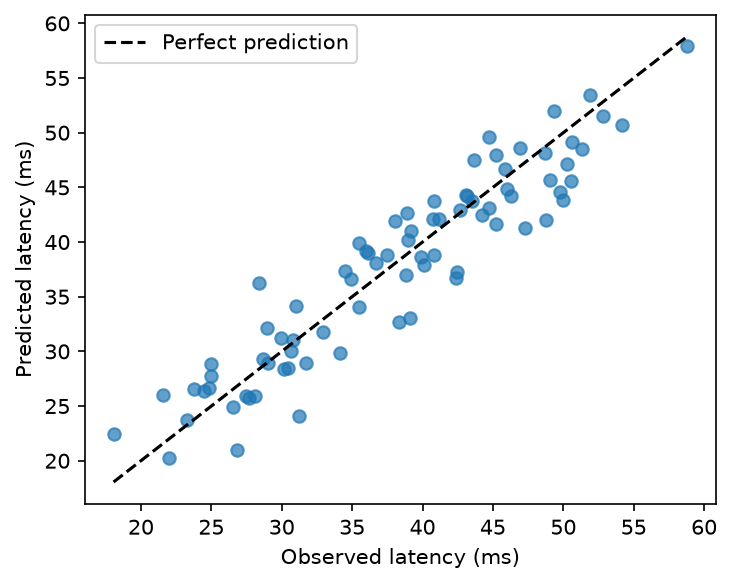
\includegraphics[height=0.28\textheight,keepaspectratio]{figures/D_student_applications_1.png}
\caption{Completed linear exercise. The model recovers the mean relationship closely, while random response noise leaves nonzero prediction errors.}\end{figure}

\subsection{Answers to the written questions}
The fitted intercept and slopes are close to 15, 3, and 2. They need not match exactly because a finite sample includes random noise. Even knowing the generating coefficients would not predict $\epsilon$; the population RMSE of the exact conditional mean is 3 ms. A finite 80-row test RMSE can differ from 3, as this run does.

\section{Logistic regression: a budget violation}
\subsection{Problem statement and data}
The second exercise generates a separate set of 800 requests with seed 42. Define
\[z=-4+0.5s+0.35q,\qquad p=\sigma(z)=\frac1{1+e^{-z}},\qquad y\sim\operatorname{Bernoulli}(p).\]
A label of 1 means a budget violation; 0 means no violation. These labels are not calculated from the first exercise's observed latencies. The sigmoid maps a real score to a probability, and the Bernoulli draw makes the outcome random.
The supplied stratified split yields 640 training and 160 test requests, with approximately equal class proportions in both sets. True probabilities are used only for simulation, not as fitted inputs.

\subsection{TODO 3: create and fit the classifier}
\begin{lstlisting}
logistic_model = LogisticRegression(max_iter=1000)
logistic_model.fit(X_logistic_train, y_logistic_train)
\end{lstlisting}
The class fits a sigmoid of a linear score. Its loss is binary log loss,
\[-y\log\hat p-(1-y)\log(1-\hat p),\]
with the library's default regularization settings. Thus this exercise does not specifically request an unpenalized fit. \code{max_iter=1000} is an optimization iteration limit, not a number of examples or a parameter fitted from data.

The completed run produces an intercept near $-4.4287$, payload slope $0.5751$, and queue slope $0.3250$. These are coefficients of log-odds, not direct probability increments. Sampling noise and regularization explain why they need not equal the generator's coefficients.

\subsection{TODO 4: extract violation probabilities}
\begin{lstlisting}
violation_probability = logistic_model.predict_proba(X_logistic_test)[:, 1]
\end{lstlisting}
For the labels 0 and 1 in this exercise, each row of the returned two-column array is
$[P(Y=0\mid x),P(Y=1\mid x)]$. The slice \code{[:, 1]} keeps all rows and selects column index 1, the second column. The resulting vector has 160 entries. Using \code{predict} here would give labels and lose the probabilities required for the next step.

\subsection{TODO 5: turn probabilities into labels}
\begin{lstlisting}
violation_prediction = (violation_probability >= 0.5).astype(int)
\end{lstlisting}
The comparison gives a Boolean array. \code{astype(int)} converts false to 0 and true to 1. Equality is explicitly assigned to class 1. The threshold 0.5 corresponds to equal false-positive and false-negative costs when correct decisions cost zero and probabilities represent risk appropriately. No threshold is fitted from the test data.

\subsection{Evaluation and answers}
\code{accuracy_score} calculates the fraction of correct decisions. The function \code{confusion_matrix}, with \code{labels=[0,1]}, returns counts with actual labels as rows and predicted labels as columns:
\begin{center}
\begin{tabular}{lrr}\toprule
&Predicted 0&Predicted 1\\\midrule
Actual 0&73&18\\
Actual 1&21&48\\\bottomrule
\end{tabular}
\end{center}
There are \textbf{18 false alarms} and \textbf{21 missed violations}. Accuracy is
\[\frac{73+48}{160}=0.75625,\]
about 75.6\%. Accuracy gives both types of error the same weight; a real application with unequal costs might use a different fixed decision rule and cost metric.
A predicted probability of 0.40 gives class 0 under this threshold. It does not guarantee no violation: a probability is an estimate of risk, not a known outcome. Even an exact model would see some violations among requests with risk 0.40.

\section*{Common mistakes to avoid}
\begin{itemize}
\item Passing targets or the simulator's true probability as input features leaks the answer.
\item Calling \code{fit} on test rows changes the experiment from evaluation to training.
\item Adding a ones column to these default model objects duplicates intercept handling.
\item Using \code{predict} when probabilities are requested prevents applying a meaningful custom cutoff.
\item Forgetting parentheses before \code{.astype(int)} can change which expression is converted.
\item Choosing a new threshold after reading test counts uses that test as development data.
\end{itemize}
The completed snippets are sufficient to run every supplied cell; no extra library, dataset, or advanced code is needed.

\section*{A practical reading guide to the five solutions}
\subsection*{Why the array dimensions matter}
For the linear exercise, \code{X_linear_train} has shape $(320,2)$ and its target has shape $(320,)$.
The first axis identifies observations; the second identifies features. A single new request still needs a
row-and-column table, for example \code{[[5.0, 3.0]]}, not just \code{[5.0, 3.0]} when calling a model that expects a matrix.
With a DataFrame, preserve the feature names too. This avoids confusing one observation with two features and
two observations with one feature.

A useful independent check of the linear answer is to calculate one prediction manually:
\[14.9261+2.9998\times5+1.9961\times3\approx35.9134\text{ ms}.\]
The fitted model should give the same value, up to displayed rounding, for a payload of 5 MB and queue of 3.
It need not match the observed latency of a newly generated request, because that request includes new noise.

\subsection*{What gets stored, and what changes state?}
The variables \code{linear_model} and \code{logistic_model} refer to estimator objects, not predictions.
Calling \code{fit} stores learned parameters inside the object. The method returns the fitted object, which is
why constructing and fitting can also be chained, although two lines are clearer for this exercise.
Calling \code{fit} a second time normally replaces the earlier fitted state; it does not mean ``continue testing.''
Calling \code{predict} returns an array without learning from its inputs.

In Python, assigning \code{second_model = linear_model} creates another reference to the same object.
It does not create an independent fit. To compare separate training runs, construct a new estimator for each.
This small programming detail matters when experiments are placed inside loops.

\subsection*{A probability table has two different axes}
The logistic probability array has one row per request and one column per learned class.
The columns approximately sum to one on each row. For a row such as $(0.60,0.40)$, the second entry is
estimated violation risk 0.40, and the explicit 0.5 rule predicts label 0.
The vectorized comparison yields a Boolean array such as \code{[False, True, False]}; converting to integer
yields \code{[0, 1, 0]}. These are decisions, not probabilities rounded for display.

An actual violation among requests predicted at risk 0.40 does not invalidate the notion of probability.
A useful assessment needs many held-out cases and asks whether probabilities and decisions perform well
across them. The confusion matrix throws away probability magnitudes, so it cannot alone assess calibration.

\subsection*{Reading estimator documentation efficiently}
Start with the \emph{Parameters} section to see choices made before fitting, then \emph{Attributes} to see values
learned by fitting, and \emph{Methods} to see operations. The distinction avoids reading a learned slope as an option
you should set manually.
Use the \href{https://scikit-learn.org/1.8/modules/generated/sklearn.linear_model.LinearRegression.html}{linear-regression reference}
and \href{https://scikit-learn.org/1.8/modules/generated/sklearn.linear_model.LogisticRegression.html}{logistic-regression reference}
for the installed course version. A similarly named method can report different quantities: a regressor's
\code{score} is $R^2$, while a classifier's is accuracy. The explicit metric calls in the worksheet avoid this ambiguity.

\subsection*{A short debugging procedure}
\begin{enumerate}
\item Run the setup and data cells before the TODO cells. A missing-name error often means execution order is wrong.
\item Replace the intentional error line, rather than inserting code below it: execution stops at the raised error.
\item Check that training X and y contain the same number of rows and the intended columns.
\item Inspect learned parameters only after fitting, and pass features alone when predicting.
\item Check prediction length, class labels, and units before interpreting a metric.
\end{enumerate}
Use a fresh kernel and run from top to bottom after finishing. A notebook can appear to work because an old
variable remains in memory even when the current cell sequence is incomplete. The worksheet's fixed settings
are intentional: extra tuning is a separate exercise and needs its own validation design.

\end{document}
